\section{The Gram-Schmidt orthogonalization procedure}

Although we have already seen some potential uses for orthogonal
bases, we have not yet seen very many examples of such bases. In this
section, we will look at the Gram-Schmidt orthogonalization procedure,
a method for turning any basis into an orthogonal one.

The basic idea is very simple: if two vectors $\vect{v}_1,\vect{v}_2$
are not orthogonal, then we can make them orthogonal by replacing
$\vect{v}_2$ by a vector of the form $\vect{w}_2 = \vect{v}_2 -
t\vect{v}_1$, for a suitable parameter $t$.
\begin{equation*}
  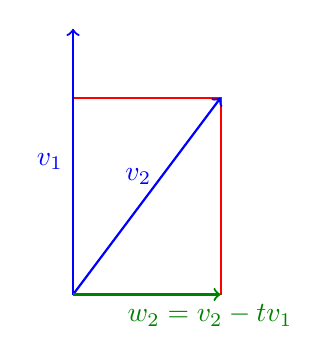
\begin{tikzpicture}[scale=1.25]
    \draw[thick,red] (1.5,0) -- (1.5,2) -- (0,2);
    \draw[thick,blue,->] (0,0) -- node[left]{$\vect{v}_1$} (0,2.7);
    \draw[thick,blue,->] (0,0) -- node[left, pos=0.6]{$\vect{v}_2$} (1.5,2);
    \draw[thick,green!50!black,->] (0,0) -- node[below right, pos=0.3]{$\vect{w}_2 = \vect{v}_2 - t\vect{v}_1$} (1.5,0);
  \end{tikzpicture}
\end{equation*}
But what is the correct value of $t$? It turns out that this value is
uniquely determined by the requirement that $\vect{v}_1$ and
$\vect{w}_2$ must be orthogonal. We calculate
\begin{equation*}
  \iprod{\vect{v}_1,\vect{w}_2}
  ~=~ \iprod{\vect{v}_1,\vect{v}_2-t\vect{v}_1}
  ~=~ \iprod{\vect{v}_1,\vect{v}_2}-t\iprod{\vect{v}_1,\vect{v}_1}.
\end{equation*}
Setting this equal to $0$ yields the unique solution
\begin{equation*}
  t = \frac{\iprod{\vect{v}_1,\vect{v}_2}}{\iprod{\vect{v}_1,\vect{v}_1}}
\end{equation*}
Note that this is exactly the same thing as the Fourier coefficient of
$\vect{v}_2$ in the direction of $\vect{v}_1$. The following
proposition summarizes what we have found so far. For consistency with
our later notation, we also rename the first basis vector $\vect{v}_1$
to $\vect{w}_1$.

\begin{proposition}{Gram-Schmidt orthogonalization procedure for 2 vectors}{gram-schmidt-2}
  Let $\set{\vect{v}_1,\vect{v}_2}$ be a basis for some subspace $W$
  of an inner product space $V$. Define vectors
  $\vect{w}_1,\vect{w}_2$ as follows:
  \begin{eqnarray*}
    \vect{w}_1 &=& \vect{v}_1, \\
    \vect{w}_2 &=& \vect{v}_2 ~-~ \frac{\iprod{\vect{w}_1,\vect{v}_2}}{\iprod{\vect{w}_1,\vect{w}_1}}\vect{w}_1.
  \end{eqnarray*}
  Then $\set{\vect{w}_1,\vect{w}_2}$ is an orthogonal basis of $W$.
\end{proposition}

\begin{example}{Gram-Schmidt orthogonalization procedure for 2 vectors}{gram-schmidt-2}
  In $\R^3$ with the usual dot product, find an orthogonal basis for
  \begin{equation*}
    \sspan\set{
      \begin{mymatrix}{c} 1 \\ 1 \\ 0 \end{mymatrix},~
      \begin{mymatrix}{c} 0 \\ 1 \\ 1 \end{mymatrix}
    }.
  \end{equation*}
\end{example}

\begin{solution}
  Let $\vect{v}_1 = \begin{mymatrix}{c} 1 \\ 1 \\ 0 \end{mymatrix}$
  and $\vect{v}_2 = \begin{mymatrix}{c} 0 \\ 1 \\ 1 \end{mymatrix}$.
  We calculate
  \begin{eqnarray*}
    \vect{w}_1
    &=& \vect{v}_1
        ~=~ \begin{mymatrix}{c} 1 \\ 1 \\ 0 \end{mymatrix},\\
    \vect{w}_2
    &=& \vect{v}_2 ~-~ \frac{\iprod{\vect{v}_1,\vect{v}_2}}{\iprod{\vect{v}_1,\vect{v}_1}}\vect{w}_1
        ~=~ \begin{mymatrix}{c} 0 \\ 1 \\ 1 \end{mymatrix}
    ~-~ \frac{1}{2}\begin{mymatrix}{c} 1 \\ 1 \\ 0 \end{mymatrix}
    ~=~ \begin{mymatrix}{c} -1/2 \\ 1/2 \\ 1 \end{mymatrix}.
  \end{eqnarray*}
  Therefore the desired orthogonal basis is
  $\set{\begin{mymatrix}{c} 0 \\ 1 \\ 1 \end{mymatrix},
    \begin{mymatrix}{c} -1/2 \\ 1/2 \\ 1 \end{mymatrix}}$.
\end{solution}

The procedure for finding an orthogonal basis of a $k$-dimensional
space is very similar. We adjust each basis vector $\vect{v}_i$ by
subtracting a suitable linear combination of previous orthogonal basis
vectors.

\begin{proposition}{Gram-Schmidt orthogonalization procedure for $k$ vectors}{gram-schmidt-k}
  Let $\set{\vect{v}_1,\ldots,\vect{v}_k}$ be a basis for some subspace $W$
  of an inner product space $V$. Define vectors
  $\vect{w}_1,\ldots,\vect{w}_k$ as follows:
  \begin{eqnarray*}
    \vect{w}_1
    &=& \vect{v}_1,
    \\
    \vect{w}_2
    &=& \vect{v}_2
        ~-~ \frac{\iprod{\vect{w}_1,\vect{v}_2}}{\iprod{\vect{w}_1,\vect{w}_1}}\vect{w}_1,
    \\
    \vect{w}_3
    &=& \vect{v}_3
        ~-~ \frac{\iprod{\vect{w}_1,\vect{v}_3}}{\iprod{\vect{w}_1,\vect{w}_1}}\vect{w}_1
        ~-~ \frac{\iprod{\vect{w}_2,\vect{v}_3}}{\iprod{\vect{w}_2,\vect{w}_2}}\vect{w}_2,
    \\
    &\vdots&
    \\
    \vect{w}_k
    &=& \vect{v}_k
        ~-~ \frac{\iprod{\vect{w}_1,\vect{v}_k}}{\iprod{\vect{w}_1,\vect{w}_1}}\vect{w}_1
        ~-~ \frac{\iprod{\vect{w}_2,\vect{v}_k}}{\iprod{\vect{w}_2,\vect{w}_2}}\vect{w}_2
        ~-~ \ldots
        ~-~ \frac{\iprod{\vect{w}_{k-1},\vect{v}_k}}{\iprod{\vect{w}_{k-1},\vect{w}_{k-1}}}\vect{w}_{k-1}.
  \end{eqnarray*}
  Then $\set{\vect{w}_1,\ldots,\vect{w}_k}$ is an orthogonal basis of $W$.
\end{proposition}

\begin{proof}
  First, it is clear that $\set{\vect{v}_1,\ldots,\vect{v}_k}$ and
  $\set{\vect{w}_1,\ldots,\vect{w}_k}$ span the same subspace, as each
  $\vect{v}_i$ is a linear combination of
  $\vect{w}_1,\ldots,\vect{w}_i$ and conversely, each $\vect{w}_i$ is
  a linear combination of $\vect{v}_1,\ldots,\vect{v}_i$. So the only
  thing we must check is that $\set{\vect{w}_1,\ldots,\vect{w}_k}$ is
  an orthogonal set.

  We prove this by induction on $k$. Assume that
  $\set{\vect{w}_1,\ldots,\vect{w}_{i-1}}$ is already known to be an
  orthogonal set. We will prove that $\vect{w}_i$ is orthogonal to all
  vectors in $\set{\vect{w}_1,\ldots,\vect{w}_{i-1}}$, thereby showing
  that $\set{\vect{w}_1,\ldots,\vect{w}_{i}}$ is an orthogonal set.
  To show that $\vect{w}_i$ is orthogonal to all vectors in
  $\set{\vect{w}_1,\ldots,\vect{w}_{i-1}}$, let $j<i$. We will show
  that $\iprod{\vect{w}_j,\vect{w}_i}=0$. We have:
  \begin{eqnarray*}
    \iprod{\vect{w}_j,\vect{w}_i}
    &=& \textstyle
        \iprod{\vect{w}_j, \vect{v}_i
        ~-~ \frac{\iprod{\vect{w}_1,\vect{v}_i}}{\iprod{\vect{w}_1,\vect{w}_1}}\vect{w}_1
        ~-~ \ldots
        ~-~ \frac{\iprod{\vect{w}_j,\vect{v}_i}}{\iprod{\vect{w}_j,\vect{w}_j}}\vect{w}_j
        ~-~ \ldots
        ~-~ \frac{\iprod{\vect{w}_{i-1},\vect{v}_i}}{\iprod{\vect{w}_{i-1},\vect{w}_{i-1}}}\vect{w}_{i-1}}
    \\
    &=& \textstyle
        \iprod{\vect{w}_j, \vect{v}_i}
        ~-~ \frac{\iprod{\vect{w}_1,\vect{v}_i}}{\iprod{\vect{w}_1,\vect{w}_1}}\iprod{\vect{w}_j,\vect{w}_1}
        ~-~ \ldots
        ~-~ \frac{\iprod{\vect{w}_j,\vect{v}_i}}{\iprod{\vect{w}_j,\vect{w}_j}}\iprod{\vect{w}_j,\vect{w}_j}
        ~-~ \ldots
        ~-~ \frac{\iprod{\vect{w}_{i-1},\vect{v}_i}}{\iprod{\vect{w}_{i-1},\vect{w}_{i-1}}}\iprod{\vect{w}_j,\vect{w}_{i-1}}
    \\
    &=& \textstyle
        \iprod{\vect{w}_j, \vect{v}_i}
        ~-~ 0
        ~-~ \ldots
        ~-~ \frac{\iprod{\vect{w}_j,\vect{v}_i}}{\iprod{\vect{w}_j,\vect{w}_j}}\iprod{\vect{w}_j,\vect{w}_j}
        ~-~ \ldots
        ~-~ 0
    \\
    &=& \iprod{\vect{w}_j, \vect{v}_i}
        ~-~ \iprod{\vect{w}_j,\vect{v}_i}
    \\
    &=& 0.
  \end{eqnarray*}
\end{proof}
